%------------------------------------------------
\section{Модели физических процессов}
%------------------------------------------------

\begin{frame}
	\frametitle{Использование моделей физических процессов.}
	\begin{enumerate}
	\item Продольная динамика -- BLonD, XSuite
	\item Поперечная динамика -- MADX, OptiM
	\item Спиновая динамика -- COSY, BMAD
	\end{enumerate}
	
	\newline
	\newline
	Использование моделирования для решения конкретных задач:
	
	Повышение критической энергии в резонансной структуре,
	расчёт внутрипучкового рассеяния, расчёт динамической апертуры, 
	влияние высших порядков на динамику, использование ВЧ различного типа, влияние импедансов,
    вычисление оси стабильного спина и частоты прецесси, декогеренция пучка, спиновые резонансы.
	
\end{frame}

\begin{frame}
	\begin{figure}
		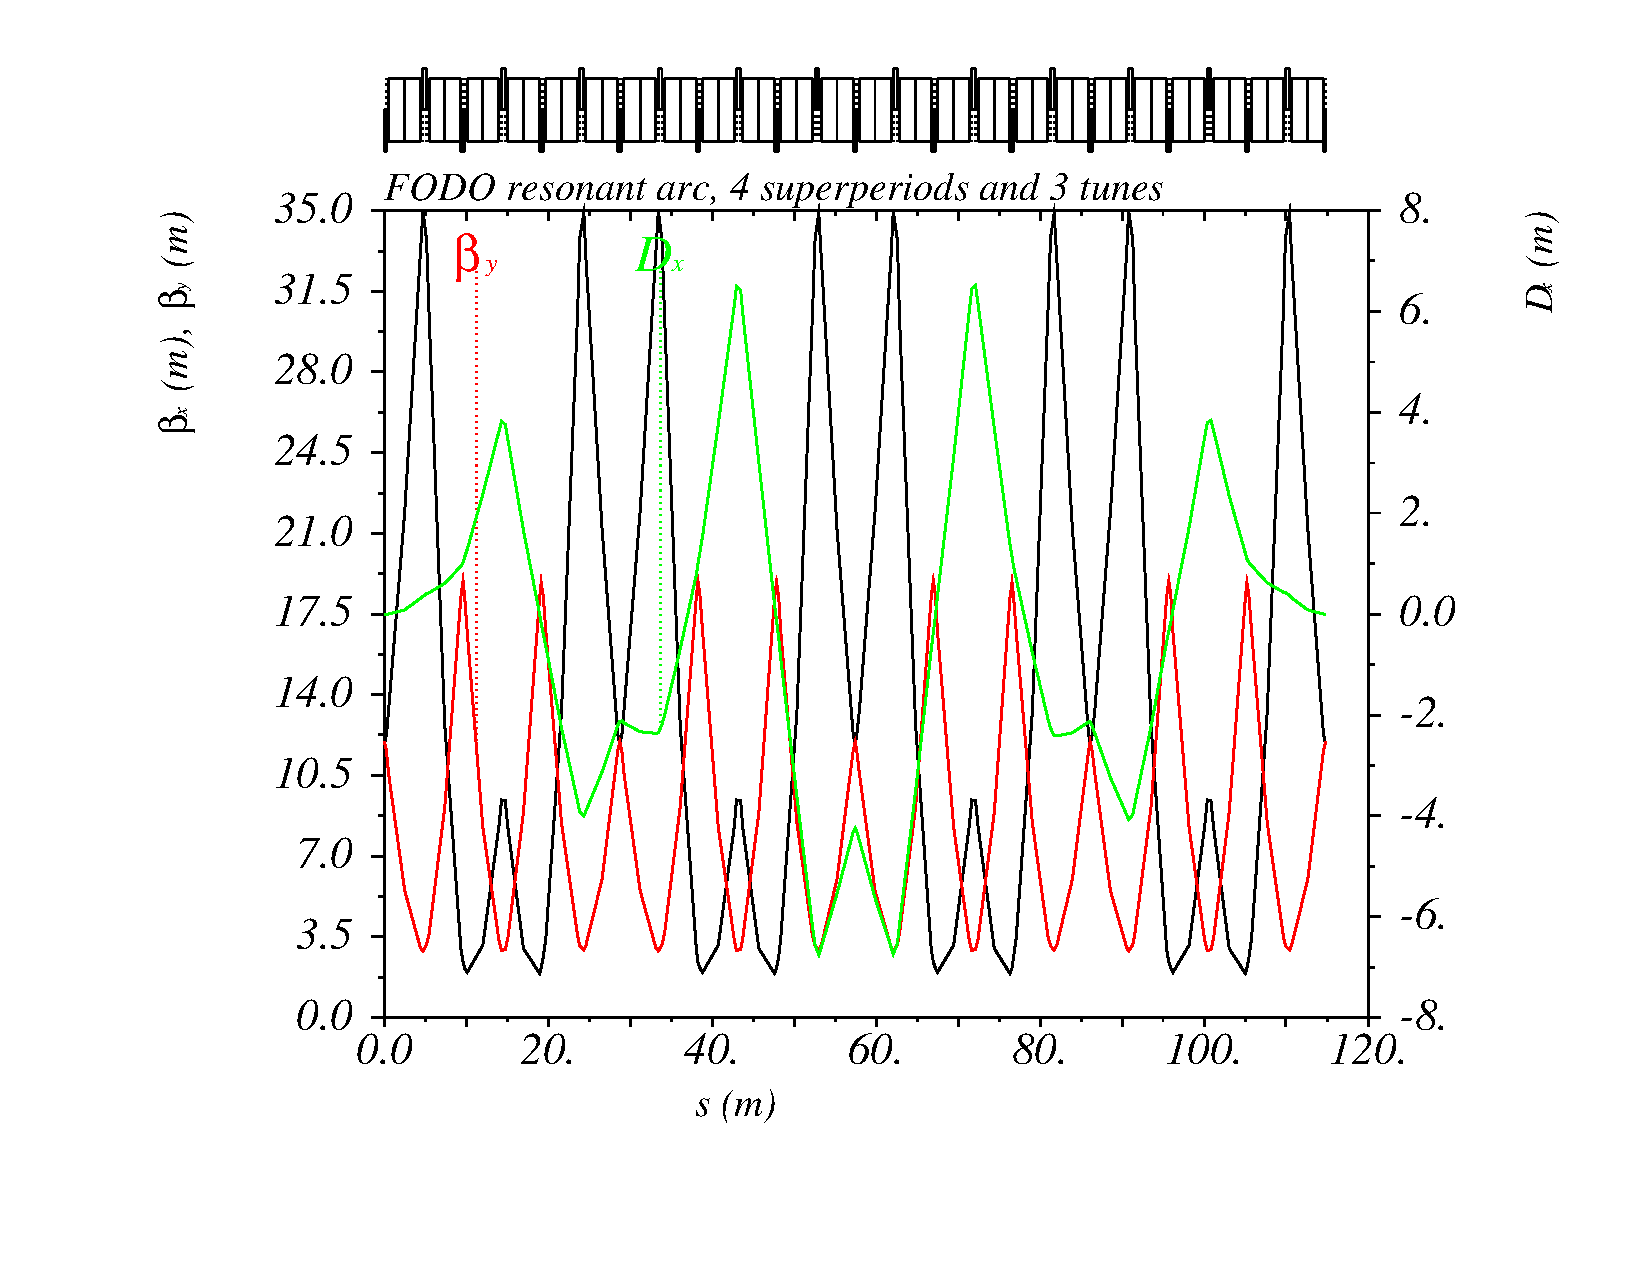
\includegraphics[width=.29\columnwidth]{images/2_twiss_fodo_resonant.pdf}
		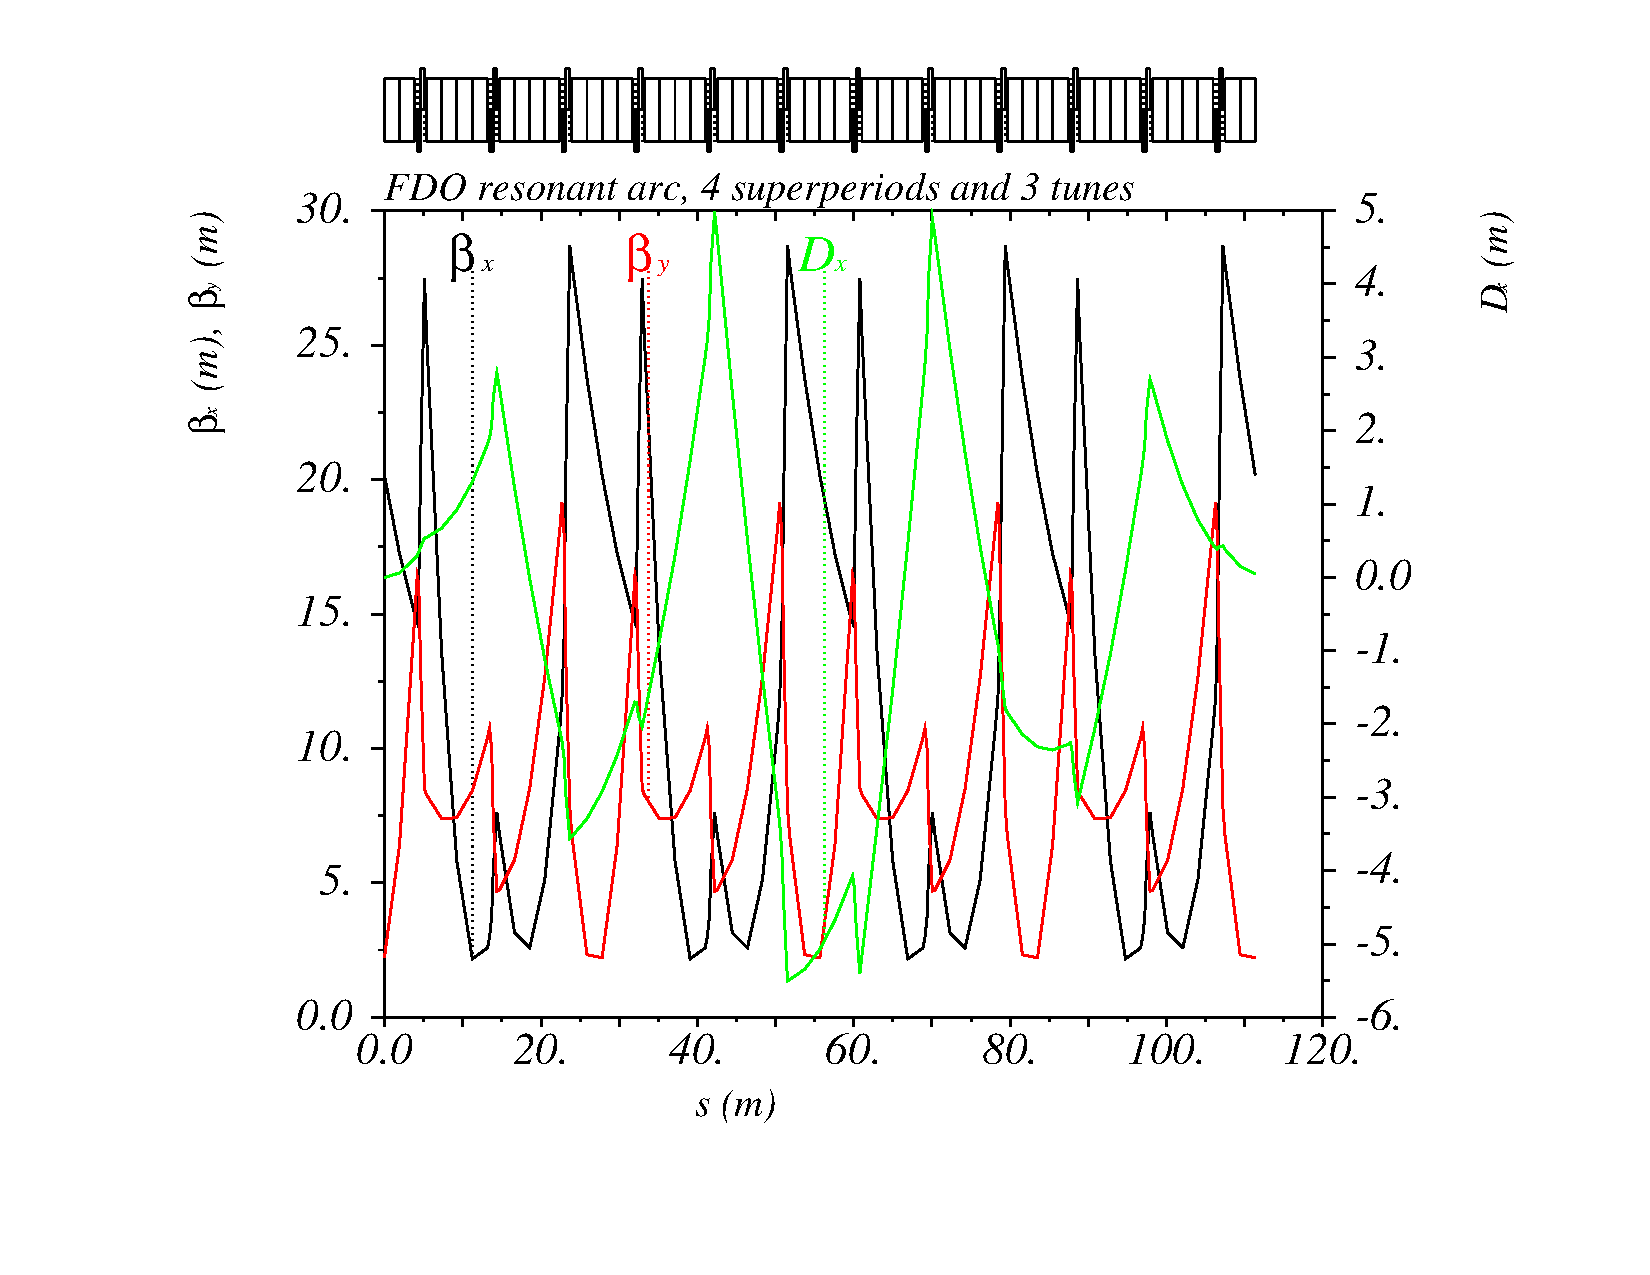
\includegraphics[width=.29\columnwidth]{images/2_twiss_fdo_resonant.pdf}
		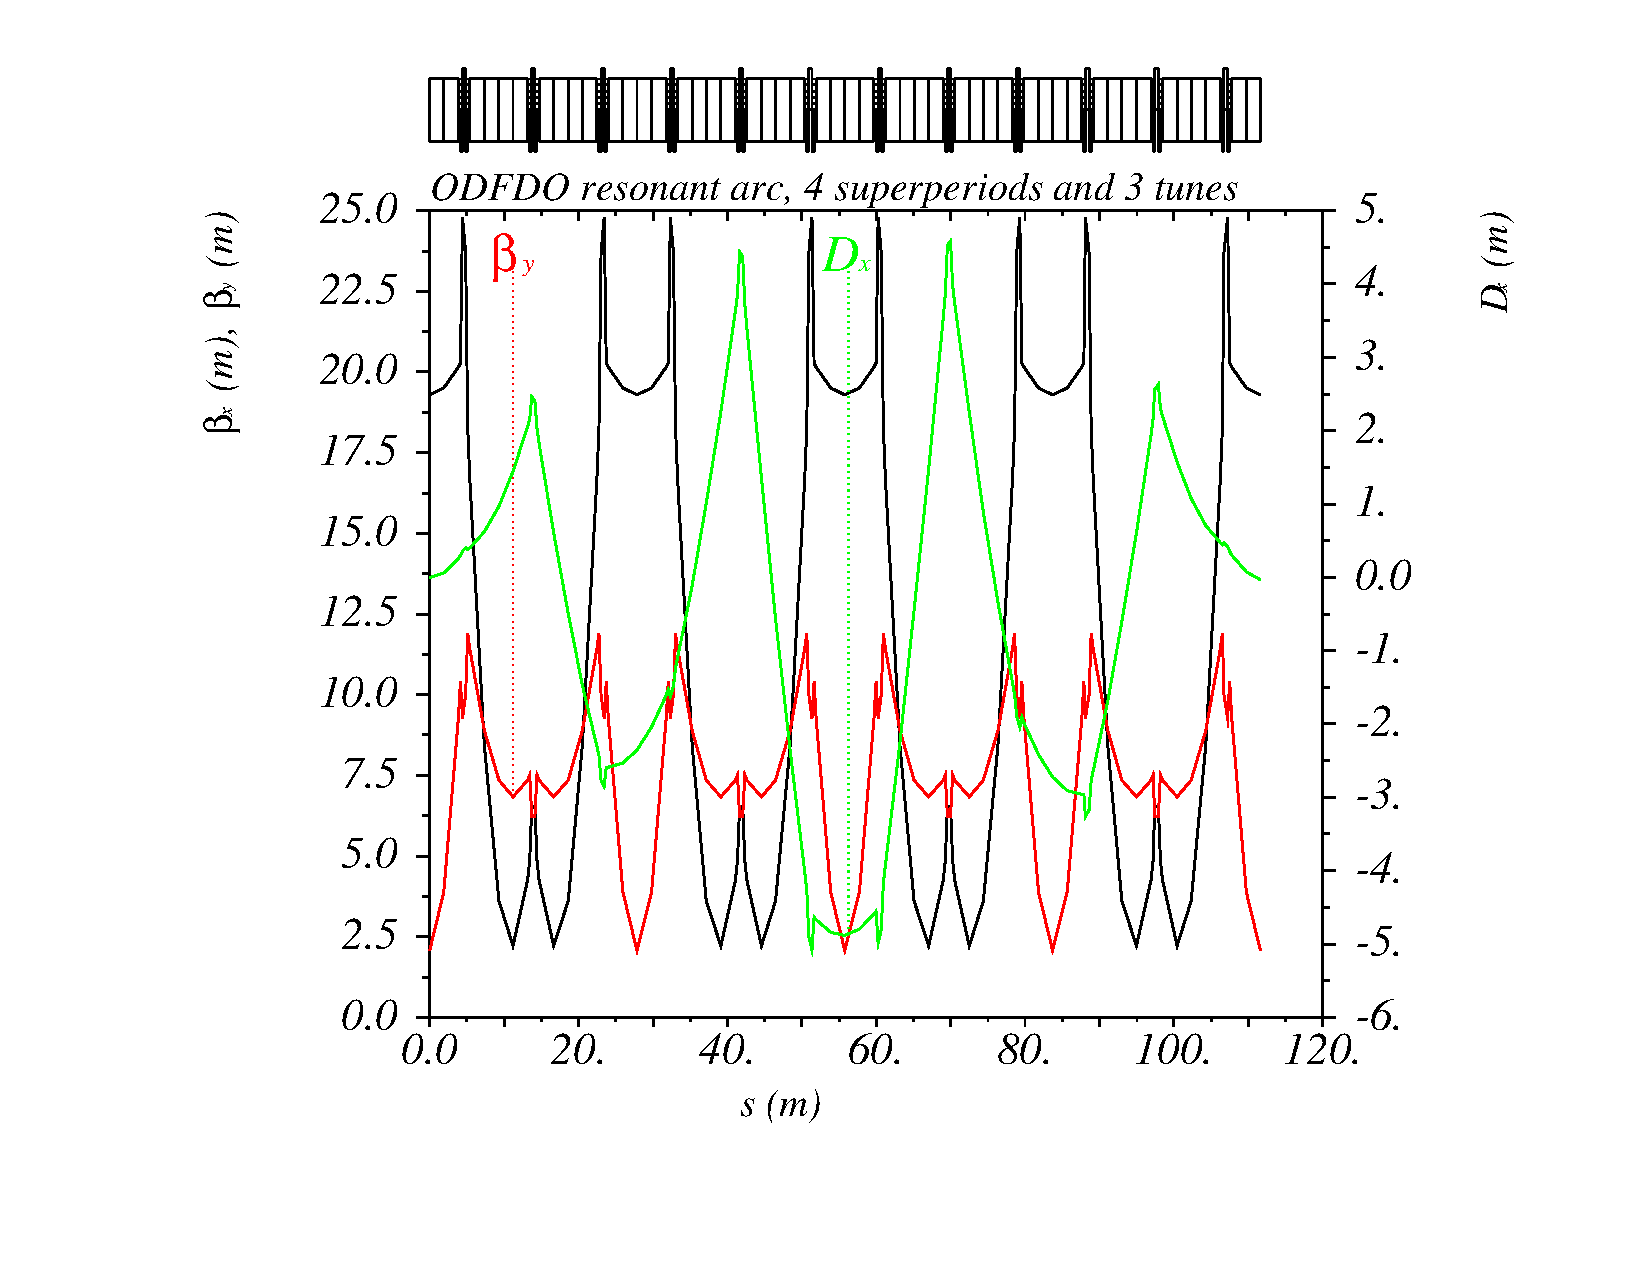
\includegraphics[width=.29\columnwidth]{images/2_twiss_odfdo_resonant.pdf}
		
		\caption{Твисс-параметры $\beta_{x,y}$, $D_{x}$. Для сигнлетной ФОДО, дублетной ФДО, триплетной ОДФДО ячеек; с  резонансной модуляцией дисперсионной функции для повышеные критической энергии.}
		\label{fig:fodo_fdo_odfdo_regular}
	\end{figure}
\end{frame}

	\begin{figure}
		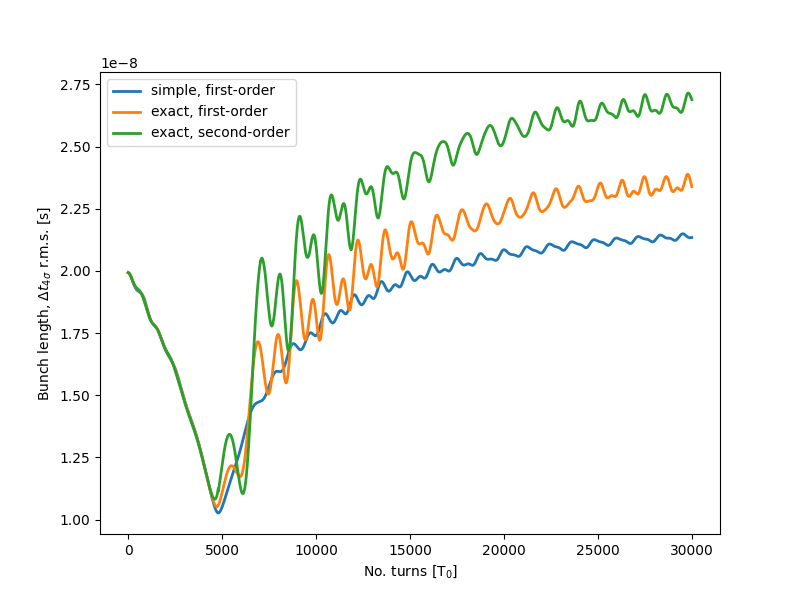
\includegraphics[width=0.32\columnwidth]{images/3_eta_beam_lenght.png}
		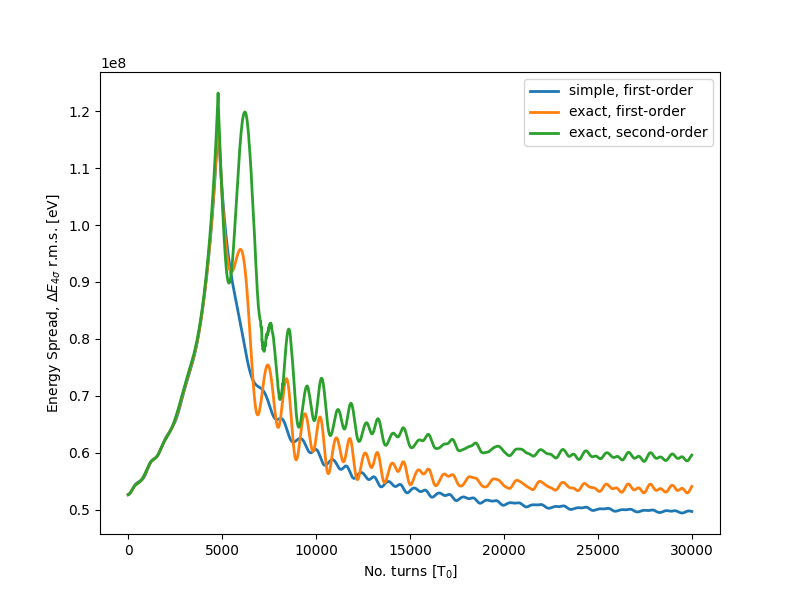
\includegraphics[width=0.32\columnwidth]{images/3_eta_energy_spread.png}
		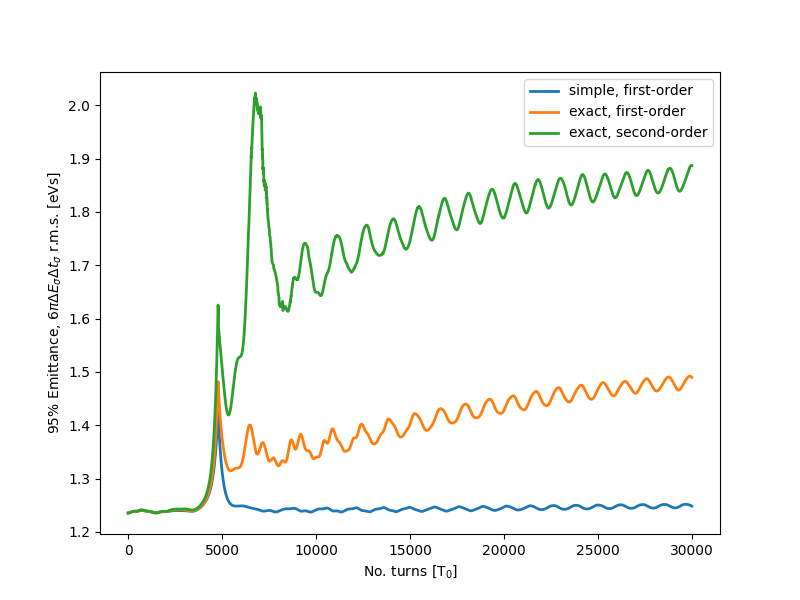
\includegraphics[width=0.32\columnwidth]{images/3_eta_emit.png}
		\caption{Зависимость a) длины cгустка, б) разброса энергии внутри сгустка, в) продольного эмиттанса от номера оборота в окрестности критической энергии при изменении энергии от $7$ до $13$ ГэВ для трёх моделей без скачка и учёта импеданса. Синяя – учёт только первого порядка $\eta=\eta_0$, ‘simple’ solver, оранжевая – $\eta=\eta_0$, ‘exact’ solver, зеленая – $\eta=\eta_0+\eta_1\delta$, ‘exact’ solver.}
		\label{fig:3_eta}
	\end{figure}

%------------------------------------------------
\begin{frame}

	\begin{figure}
		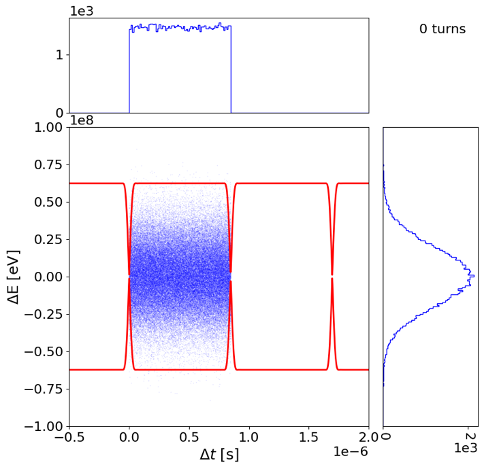
\includegraphics[width=.4\columnwidth]{images/3_BB_PS_near_tr}
		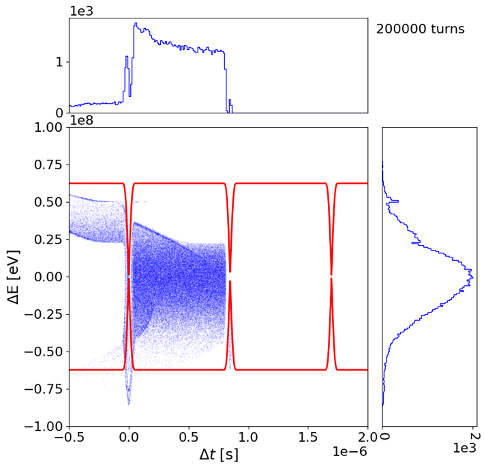
\includegraphics[width=.4\columnwidth]{images/3_BB_PS_near_tr_2}
		\caption{Фазовая плоскость при удержании пучка внутри ВЧ-барьера. Слева – начальное распределение, справа – распределение после $2\times{10}^5 оборотов$.}
		\label{fig:BB_PS_near_tr}
	\end{figure}

\end{frame}

\begin{frame}
	
	\begin{figure}
		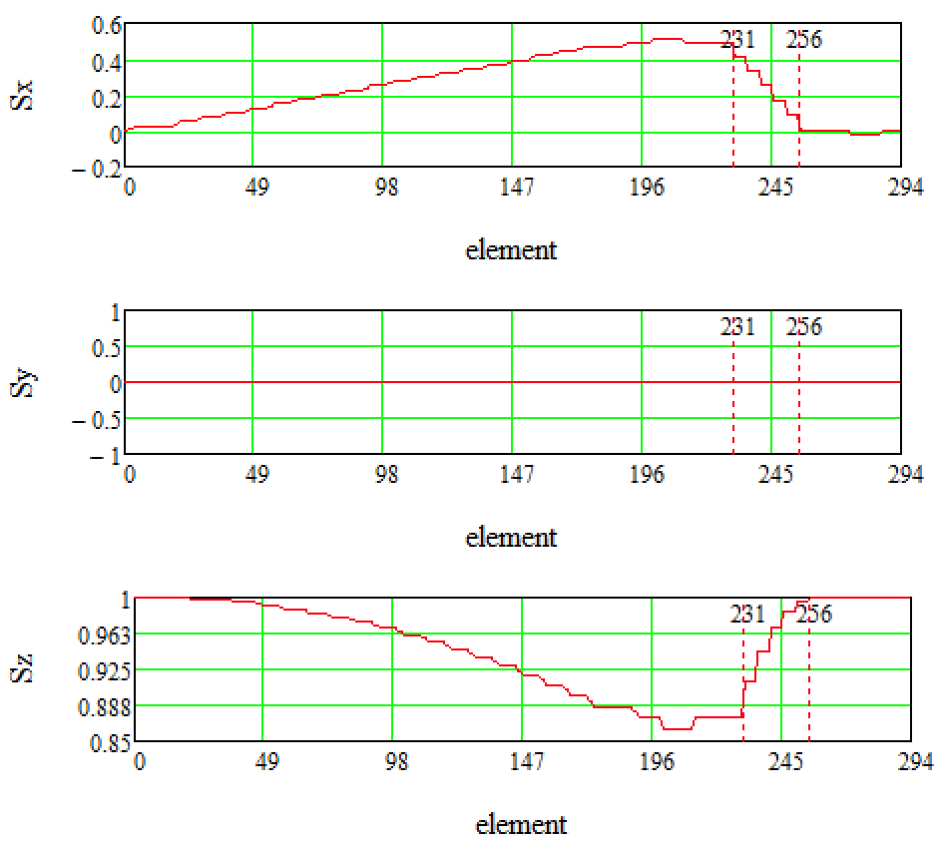
\includegraphics[width=.45\columnwidth]{images/spin}
		\caption{Режим квази-замороженного спина для половины кольца в поэлементном моделировании.}
	\end{figure}
	
\end{frame}

